% -----------------------------------------------------------------
% Vorlage fuer Ausarbeitungen von
% Bachelor- und Masterarbeiten am ISS
% 
% Template for written reports or master theses at the ISS
% 
% For use with compilers pdflatex or latex->dvi2ps->ps2pdf.
%
% -----------------------------------------------------------------
% README, STUDENT USERS:
% We highly appreciate students using this template _AS IS_,period. 
% The document provides adjustable document preferences, 
% student information settings and typography definitions. Look for
% code delimited by *** ***
%
% The short explanation: it's the ISS common standard and 
% 	it's battle tested.
% The long explanation: 
%	We do not want you to go through the document and tweak the 
%	package options, layout parameters and line skips here and 
%	there and waste hours. We are providing this template such 
%	that you can fully concentrate on filling in the much more 
%	important _contents_ of your thesis.
%
% If you have serious needs on extra packages or design 
% modifications, talk to your supervisor _before_ modifying 
% the template.
% Similarly, we're happy if you give your supervisor a hint on any 
% errors in this template.
%
% -----------------------------------------------------------------
% History:
% Jan Scheuing,   04.03.2002
% Markus Buehren, 20.12.2004
% last changes:   10.01.2008 (removed unused packages), 
% 		07.08.2009 (added IEEEtran_LSS.bst file)
% 		02.05.2011 removed matriculation number from cover page
% Martin Kreissig, 25.01.2012: all eps/ps parts removed for 
% 				pdflatex to work properly
% Peter Hermannstaedter, 14.08.2012: fusion of versions for 
% 		latex/dvi/ps/pdf and pdflatex, additional comments,
% 		unification of document flags and student options
% Florian Liebgott, 12.03.2015: bug fixes, removal of obsolete options,
%		switch to UTF-8
% Florian Liebgott, 20.05.2015: fixed encoding problem on title page
% Florian Liebgott, 24.01.2017: changed deprecated font commands (like
%		\sl) to up-to-date commands to be compatible with
%		current TeX distributions.
%
% -----------------------------------------------------------------
% If you experience any errors caused by this template, please
% contact Florian Liebgott (florian.liebgott@iss.uni-stuttgart.de)
% or your supervisor, so we can fix the errors.
% -----------------------------------------------------------------


\documentclass[12pt,DIV14,BCOR12mm,a4paper,footinclude=false,headinclude,parskip=half-,twoside,openright,cleardoublepage=empty,toc=index,bibliography=totoc,listof=totoc]{scrreprt}
% encoding needs to be defined here, otherwise umlauts on the titelpage won't work.
\usepackage[utf8]{inputenc}
%
%
%
% *****************************************************************
% -------------------> document preferences here <-----------------
% *****************************************************************
% Uncomment the settings you like and comment the settings you don't
% like.

% Language: 
% affects generic titles, Figure term, titlepage and bibliography
% (Note:if you switch the language, compile tex and bib >2 times)
\def \doclang{english} 	% For theses/reports in English
%\def \doclang{german} 		% For theses/reports in German

% Hyperref links in the document:
\def \colortype{color} % links with colored text
%\def \colortype{bw} 	% plain links, standard text color (e.g. for print)
%\def \colortype{boxed} % links with colored boxes
% *****************************************************************
%
%
%
% *****************************************************************
% --------------> put student information here <------------------
% *****************************************************************
% Please fill in all items denoted by "to be defined (TBD)"
\def \deworktitle{Pattern Recognition}        % German title/translation
\def \enworktitle{Statistical Signal Processing}        % English title/translation
\def \tutor{Lukas Mauch}
\def \student{Yuxin Liu, Shanqi Yang, Qianqian Wei}
\def \worksubject{LAB}  % type and number (S/Dxxxx) of your thesis
\def \startdate{Date of work begin TBD}
\def \submission{Date of submission TBD}
\def \signagedate{TBD Date of sign.}   % Date of signature of declaration on last page
\def \keywords{Prostate Cancer Segmentation,
	Speaker Recognition}
\def \abstract{Abstract: Pattern recognition deals with a wide variety of problems. Methods
	of pattern recognition are prevalent in applications, such as the facial recognition
	and speech recognition systems. This pattern recognition lab includes two tasks,
	prostate cancer segmentation and speaker identification, which cope with medical
	imaging area and authentication field, respectively. The prostate cancer segmentation
	aims to detect the cancerous prostate area automatically, which saves cost
	and time for patients and medical workers. The speaker identification system can
	be used in several apps for authentication, like online banking, email services. As a
	consequence, the prostate cancer segmentation achieves an acceptable performance,
	and speaker identification system performs greatly.}

% *****************************************************************
%


\usepackage{amsmath}
\usepackage{amsfonts}
\usepackage{ifthen}
\ifthenelse{\equal{\doclang}{german}}{
	\usepackage[ngerman]{babel} %german version
	\def \maintitle{\deworktitle}
	\def \translatedtitle{\enworktitle}
	% set , to decimal and . to thousands separator, if German language is used
	\DeclareMathSymbol{,}{\mathord}{letters}{"3B}
	\DeclareMathSymbol{.}{\mathpunct}{letters}{"3A}
	}{
	%english version
	\def \maintitle{\enworktitle}
	\def \translatedtitle{\deworktitle}
	}
\usepackage{txfonts} % Times-Fonts
\usepackage[T1]{fontenc}
\usepackage{color}
\usepackage[headsepline]{scrpage2} % Headings

\usepackage{graphicx}
\usepackage[format=hang]{caption}       % for hanging captions
\usepackage{subfig}                     % for subfigures
\usepackage{wrapfig}                    % for figures floating in text, alternatively you can use >>floatflt<<
\usepackage{booktabs}                   % nice looking tables (for tables with ONLY horizontal lines)

%%%%% Tikz / PGF - drawing beautiful graphics and plots in Latex
% \usepackage{tikz}
% \usetikzlibrary{plotmarks}              % larger choice of plot marks
% \usetikzlibrary{arrows}                 % larger choice of arrow heads
% % ... insert other libraries you need
% \usepackage{pgfplots}
% % set , to decimal and . to thousands separator for plots, if German language is used
% \ifthenelse{\equal{\doclang}{german}}{
% \pgfkeys{/pgf/number format/set decimal separator={,}}
% \pgfkeys{/pgf/number format/set thousands separator={.}}
% }{}
%%%%%%

\ifthenelse{\equal{\colortype}{color}}{
	% colored text version:
	\usepackage[colorlinks,linkcolor=blue]{hyperref}
	\newcommand{\bugfix}{\color{white}{\texttt{\symbol{'004}}}} % Bug-Fix Umlaute in Verbatim
}{
	\ifthenelse{\equal{\colortype}{boxed}}{
		% colored box version:
		\usepackage{hyperref}
		\newcommand{\bugfix}{\color{white}{\texttt{\symbol{'004}}}} % Bug-Fix Umlaute in Verbatim
	}{
		% monochrome version:
		\usepackage[hidelinks]{hyperref}
		\newcommand{\bugfix}{\color{white}{\texttt{\symbol{'004}}}} % Bug-Fix Umlaute in Verbatim
	}
}

% Layout and Headings
\pagestyle{scrheadings}
\automark{chapter}
\clearscrheadfoot
\lehead[]{\pagemark~~\headmark}
\rohead[]{\headmark~~\pagemark}
\renewcommand{\chaptermark}[1]{\markboth {\normalfont\slshape \hspace{8mm}#1}{}}
\renewcommand{\sectionmark}[1]{\markright{\normalfont\slshape \thesection~#1\hspace{8mm}}}
\addtolength{\textheight}{15mm}
\parindent0ex
\setlength{\parskip}{5pt plus 2pt minus 1pt}
\renewcommand*{\pnumfont}{\normalfont\slshape} % Seitenzahl geneigt
\renewcommand*{\sectfont}{\bfseries} % Kapitelueberschrift nicht Helvetica

% Settings for PDF document
\pdfstringdef \studentPDF {\student} 
\pdfstringdef \worktitlePDF {\maintitle}
\pdfstringdef \worksubjectPDF {\worksubject}
\hypersetup{pdfauthor=\studentPDF, 
            pdftitle=\worktitlePDF,
            pdfsubject=\worksubjectPDF}

% Title page
\titlehead{
	
\includegraphics[width=20mm]{university-logo}
	\hspace{6mm}
	\ifthenelse{\equal{\doclang}{german}}{
		\begin{minipage}[b]{.6\textwidth}
		{\Large Universit\"at Stuttgart } \\
		Institut f\"ur Signalverarbeitung und Systemtheorie\\
		Professor Dr.-Ing. B. Yang \vspace{0pt}
		\end{minipage}
	}{
		\begin{minipage}[b]{.6\textwidth}
		{\Large University of Stuttgart } \\
		Institute for Signal Processing and System Theory\\
		Professor Dr.-Ing. B. Yang \vspace{0pt}
		\end{minipage}
	}
	\hspace{1mm}
	
\includegraphics[width=28mm]{isslogocolor}
}
\subject{\worksubject\vspace*{-5mm}} % Art und Nummer der Arbeit
\title{\maintitle}%\\ \Large{\subtitle}}
\subtitle{\translatedtitle}
\author{
\large
  \ifthenelse{\equal{\doclang}{german}}{
  \begin{tabular}{rp{7cm}}
    \Large 
    Autor:      & \Large \student \vspace*{2mm}\\
    Ausgabe:    & \startdate \\
    Abgabe:     & \submission \vspace*{3mm}\\
    Betreuer:   & \tutor \vspace*{2mm}\\
    Stichworte: & \keywords
  \end{tabular}
  }{
  \begin{tabular}{rp{7cm}}
    \Large 
    Author:             & \Large \student \vspace*{2mm}\\
    Date of work begin: & \startdate \\
    Date of submission: & \submission \vspace*{3mm}\\
    Supervisor:         & \tutor \vspace*{2mm}\\
    Keywords:           & \keywords
  \end{tabular}
  }
  \bugfix
}
\date{}
\publishers{\normalsize
  \begin{minipage}[t]{.9\textwidth}
    \abstract
  \end{minipage}
}

\numberwithin{equation}{chapter} 
\sloppy 

%
%
%
% *****************************************************************
% --------------> put typography definitions here <----------------
% *****************************************************************
% colors
\definecolor{darkblue}{rgb}{0,0,0.4}

% declarations
\newcommand{\matlab}{\textsc{Matlab}\raisebox{1ex}{\tiny{\textregistered}} }
% Integers, natural, real and complex numbers
\newcommand{\Z}{\mathbb{Z}}
\newcommand{\N}{\mathbb{N}}
\newcommand{\R}{\mathbb{R}}
\newcommand{\C}{\mathbb{C}}
% expectation operator
\newcommand{\E}{\operatorname{E}}
% imaginary unit
\newcommand{\im}{\operatorname{j}}
% Euler's number with exponent as parameter, e.g. \e{\im\omega}
\newcommand{\e}[1]{\operatorname{e}^{\,#1}}
% short command for \operatorname{}
\newcommand{\op}[1]{\operatorname{#1}}

% unknown hyphenation rules
\hyphenation{Im-puls-ant-wort Im-puls-ant-wort-ko-ef-fi-zien-ten
Pro-gramm-aus-schnitt Mi-kro-fon-sig-nal}
% *****************************************************************
%
\begin{document}

% title and table of contents
\pagenumbering{alph}
\maketitle
\cleardoublepage
\pagenumbering{roman} % roman numbering for table of contents
\tableofcontents
\cleardoublepage
\setcounter{page}{1}
\pagenumbering{arabic} % arabic numbering for rest of document

% *****************************************************************
% -------------------> start writing here <------------------------

\chapter{Introduction}
\section{Evaluation}
In last section we built up our generation and identification model and in order to get best performance of the model, It is necessary to analysis the hyper-parameters. We applied grid-search method on the parameters including SNR (Signal Noise Ratio), Maximum iterations and covariance types. All of these parameters may have significant impact on the model performance.
\subsection{Signal Noise Ratio Analysis}
In the previous section , we have implemented a voice detector to separate voiced frames and unvoiced frames, its mathematic equation follows . Now the threshold of the voice detector is going to ensured according to cross-validation performance. 

\begin{table}
    \centering
    \caption{Detection Rate with different SNR threshold}
    \label{SNR}
    \begin{tabular}{lccccc}
        \toprule
         & $\gamma=1$ & $\gamma=5 $& $\gamma=10 $& $\gamma=50$ & $\gamma=100 $\\
        \midrule
        Expected Detection Rate & 0.994117 & 0.994705 &  0.995294 & 0.993529 & 0.991764\\
        \bottomrule
    \end{tabular}
\end{table}

As it is seen in the Table.\ref{SNR}, the model has best Detection Rate when SNR threshold $\gamma = 10$.

\subsection{Convergence Analysis}
In previous section, new model coefficients are generated using EM algorithm. However the model doesn't converge with only one iteration. Then we tuned the maximum iterations of Gaussian Mixture Model , aiming to figure out when convergence achieved and its impact on detection rate. See the Table.\ref{fullcov}, we take expected value among cross validation sets under different maximum iteration. When only one iteration, the GMM model seems to be underfitting because both detection rate and log-PDF are low. With maximum iteration increasing, both detection rate and log-PDF raise. When maximum iteration equals to 3, expected detection rate reaches the peak, and afterward GMM seems to be overfitting that detection rate goes down with log-PDF arising. Due to that GMM api from Sklearn will automatically report convergence, so we know that the model is converged until maximum iteration is close to 100, but it is definitely overfitting.

\begin{table}
	\centering
	\caption{Performance \& Convergence Analysis with FULL covariance type}
	\label{fullcov}
	\begin{tabular}{lccc}
		\toprule
& Expected Detection Rate & Expected Log-PDF & Cross\_Valid Time (minutes) \\
\midrule
$Max\_iter=1$ & 0.995294 & -47.724 &  39.2 \\
$Max\_iter=2$ & 0.997058 & -52.958 &  34.5 \\
$Max\_iter=3$ & 0.997647 & -53.023 &  38.8 \\
$Max\_iter=4$ & 0.997058 & -53.031 &  37.1 \\
$Max\_iter=5$ & 0.997058 & -53.021 &  43.2 \\
$Max\_iter=6$ & 0.995294 & -53.000 &  46.0 \\
$Max\_iter=7$ & 0.994117 & -52.966 &  60.0 \\
$Max\_iter=8$ & 0.992352 & -52.935 &  57.1 \\
$Max\_iter=9$ & 0.991176 & -52.924 &  59.2 \\
$Max\_iter=10$ & 0.991764 & -52.930 &  61.5 \\
\bottomrule
	\end{tabular}
\end{table}

\begin{table}
	\centering
	\caption{Performance \& Convergence Analysis with DIAGONAL covariance type}
	\label{diagcov}
	\begin{tabular}{lccc}
		\toprule
		& Expected Detection Rate & Expected Log-PDF & Cross\_Valid Time (minutes) \\
		\midrule
		$Max\_iter=1$ & 0.864117 & -36,822 &  11.4 \\
		$Max\_iter=2$ & 0.93 & -36.606 &  15.1 \\
		$Max\_iter=3$ & 0.957058 & -36.651 &  16.7 \\
		$Max\_iter=4$ & 0.958235 & -37.744 &  17 \\
		$Max\_iter=5$ & 0.965882 & -36.816 &  18.7 \\
		$Max\_iter=6$ & 0.97 & -36.870 &  21.2 \\
		$Max\_iter=7$ & 0.971176 & -36.921 &  21.3 \\
		$Max\_iter=8$ & 0.968235 & -36.969 &  21.1 \\
		$Max\_iter=9$ & 0.972352 & -37.006 &  19.8 \\
		$Max\_iter=10$ & 0.972941 & -37.031 &  20.9 \\
		\bottomrule
	\end{tabular}
\end{table}

But only tunned maximum iteration is not sufficient for analyzing convergence and performance, we also put the covariance types into consideration. Table.\ref{fullcov} implements with FULL covariance type and Table.\ref{diagcov} implements with DIAGONAL covariance. We make a contrast with both covariance types, the calculation time of FUll covariance is 2 or 3 times of DIAGONAL covariance's time. It is easy to think over that FULL covariance has more coefficients than DIAGONAL covariance so it will takes more time when FULL covariance. Furthermore, we plot the variation of detection rates of two covariance types. 

\begin{figure}
	\centering
	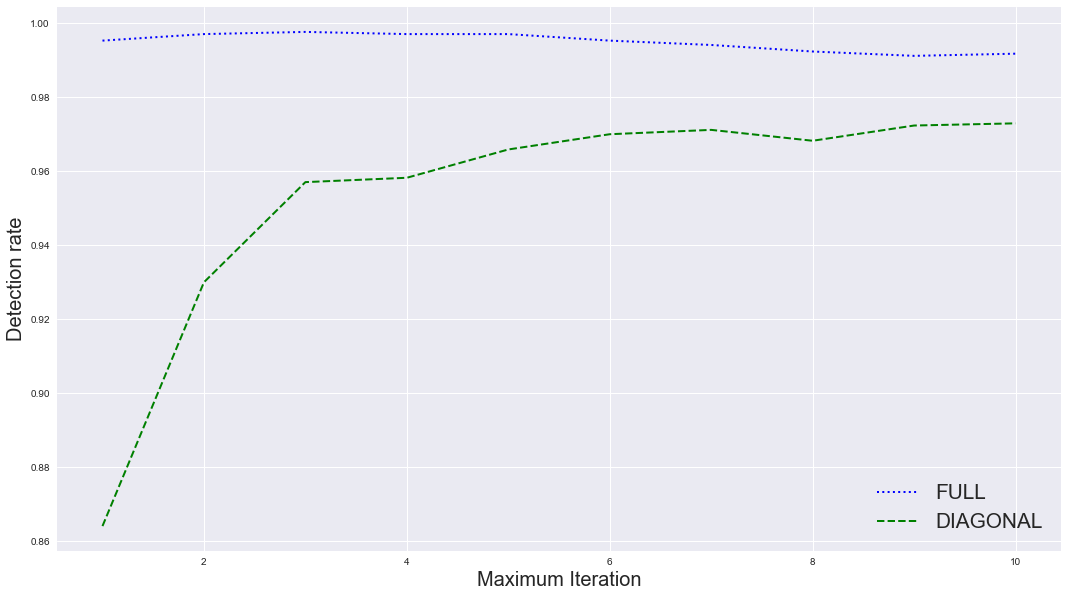
\includegraphics[scale=0.4]{image/detect_cov}
	\caption{ Variation of Detection Rate with different covariance types in models}
	\label{detect_cov}
\end{figure}
Figure.\ref{detect_cov} illustrates that FULL covariance has faster convergence speed and better performance than DIAGONAL covariance does, detection rate of DIAGONAL covariance has a gap 2\% between detection rate of FULL covariance when both reach peak plain. To figure out why, Figure.\ref{cov_type} illustrates covariance types have the different effects on the GMM model distribution.

\begin{figure}
	\centering
	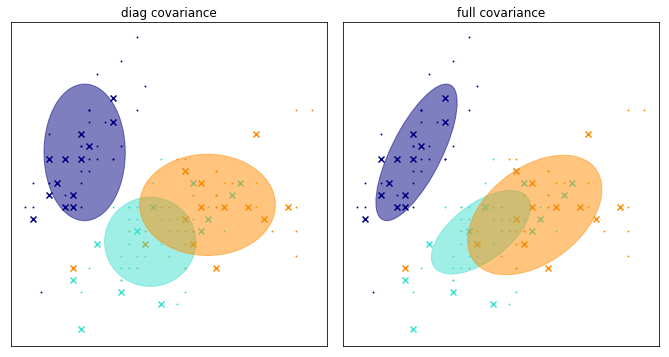
\includegraphics[scale=0.5]{image/cov_type}
	\caption{ GMM distribution Different Covariance Types}
	\label{cov_type}
\end{figure}

From the Figure.\ref{cov_type}, FULL covariance type may lead to a sloped ellipse but DIAGONAL covariance lead to an upright ellipse distribution. So our case, few GMM model with FULL covariance type can fit our voice dataset but the same number of models is not sufficient for DIAGONAL covariance type. One sloped ellipse distribution can be made up of several regular and upright ellipses. In conclusion, FULL covariance type fit the irregularly shaped dataset better and lead to faster convergence but it will cost more calculation time than DIAGONAL covariance type dose.

\subsection{Result Evaluation}
Finally, we find out the parameters with best performance lets see how good it is. We plot the confusion matrix of 10-cross-validation of 170 speakers, see the Figure.\ref{con_mat} , only 4 samples of 1700 samples are misidentified. 

\begin{figure}
	\centering
	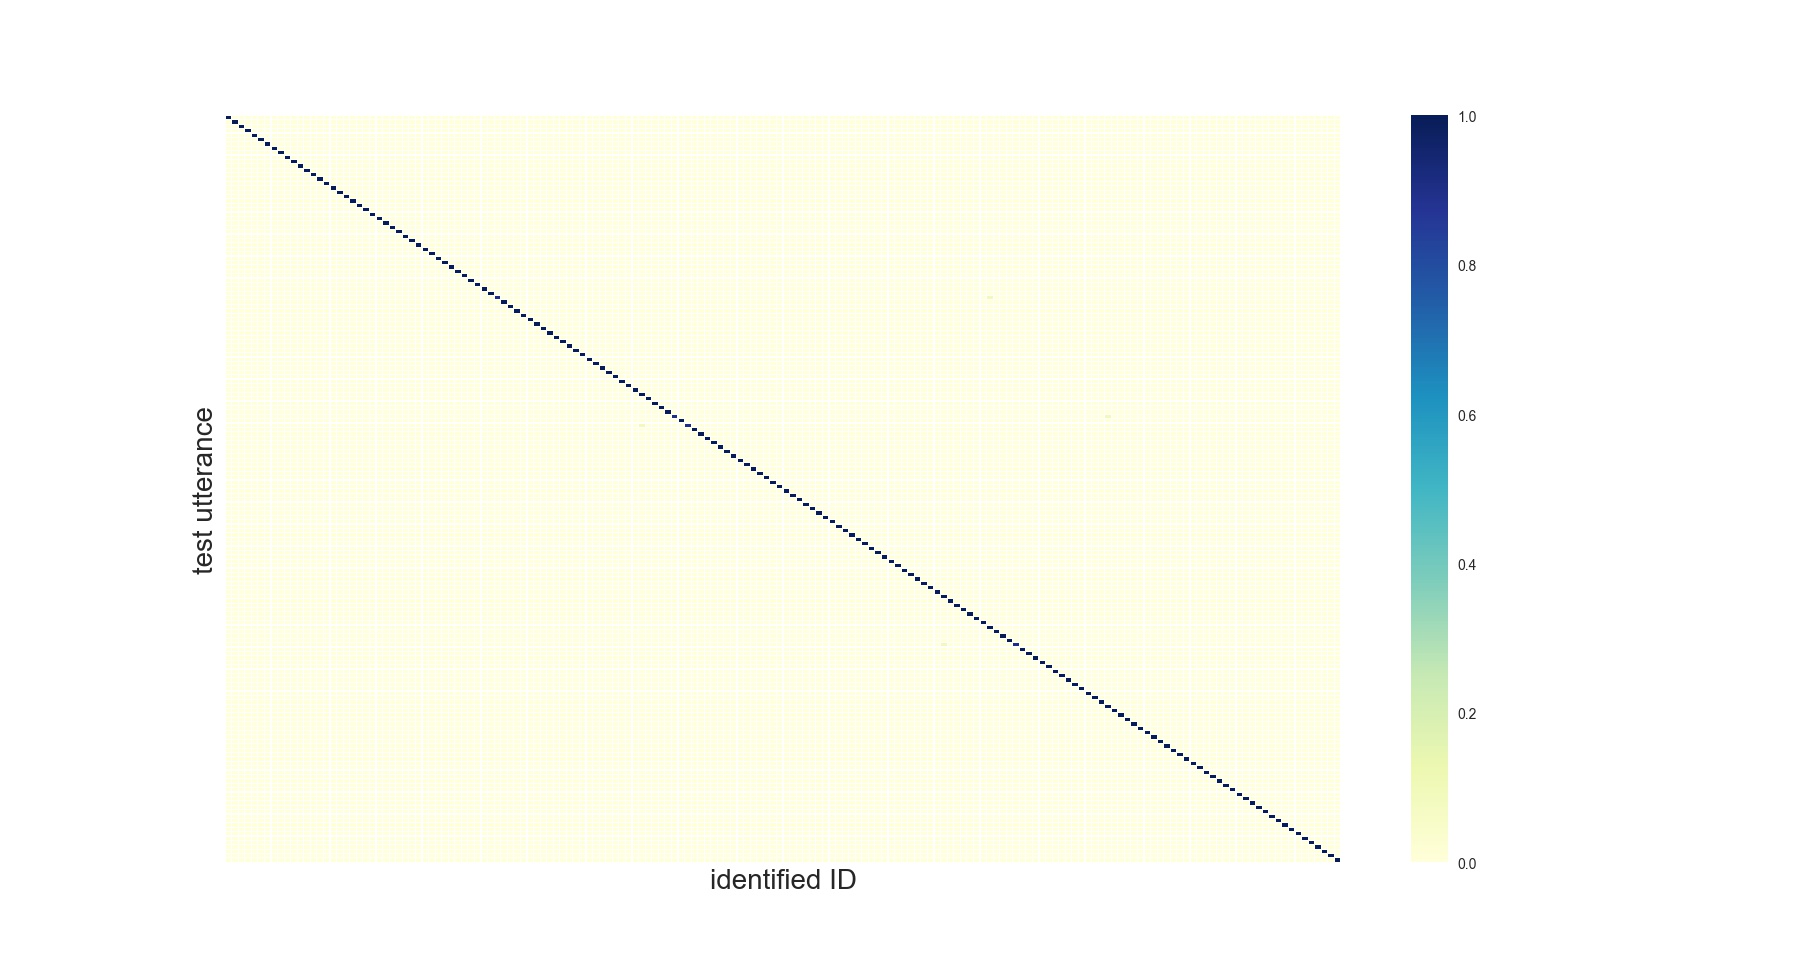
\includegraphics[scale=0.3]{image/confusion_matrix}
	\caption{Confusion Matrix Plot of 170 Speakers}
	\label{con_mat}
\end{figure}

\begin{table}
	\centering
	\caption{Details of the misidentification}
	\label{misid}
	\begin{tabular}{lcc}
		\toprule
		& True & False  \\
		\midrule
		Crossvalidation\ 4 & mbwm0 & mklt0 \\
		Crossvalidation\ 4 & fjmg0 & fadg0 \\
		Crossvalidation\ 5 & mrrk0 & mcrc0 \\
		Crossvalidation\ 9 & fgjd0 & fcau0 \\
		\bottomrule
	\end{tabular}
\end{table}

Due to the Table.\ref{misid}, we found no gender misidentified(one gender misidentified to the other one) and our custom voice (last 2 speakers) are both identified correctly.In addition, We observe from cross validations with different parameters that most misidentified speakers are male, so we suppose that low frequency voice (the voice from most male has lower frequency than from most female) is a little bit difficult to be identified correctly in our model, it can be improved in future work.

\section{Enhancement}
From the content of previous sections, we have achieved high accuracy of Speaker identification among known speakers or we could see speakers registered in our model. However this model is not realistic because if there is an unknown speaker, the model will pair the unknown speaker to one of registered ID and it is obviously incorrect. So unregistered speaker identification is always tough challenge of general Speaker Identification. In order to solve that, we used OSTI-SI (Open-set,Text-independent Speaker Identification), evaluated the error rate and finally optimal the performance of Identification model.

Before start, we selected first 3 files of TIMIT's Training set ($dr1,dr2,dr3$) as unknown speakers' voice set. Table.\ref{enh_data} shows the people number, gender distribution of selected unknown speakers and in contrast with registered speakers.

\begin{table}
	\centering
	\caption{Configuration of the OSTI-SI Dataset}
	\label{enh_data}
	\begin{tabular}{lcc}
		\toprule
		& Female & Male  \\
		\midrule
		Registered Speakers & 64 & 106 \\
		Non-registered Speakers & 66 & 124 \\
		\bottomrule
	\end{tabular}
\end{table}

The process of the open-set speaker Identification is shown in the Figure.\ref{OSIE}. The most important part is to set up threshold of comparison between registered and unregistered speaker. We introduced the ratio test between registered model and UBM's probability density function(PDF).

\begin{figure}
	\centering
	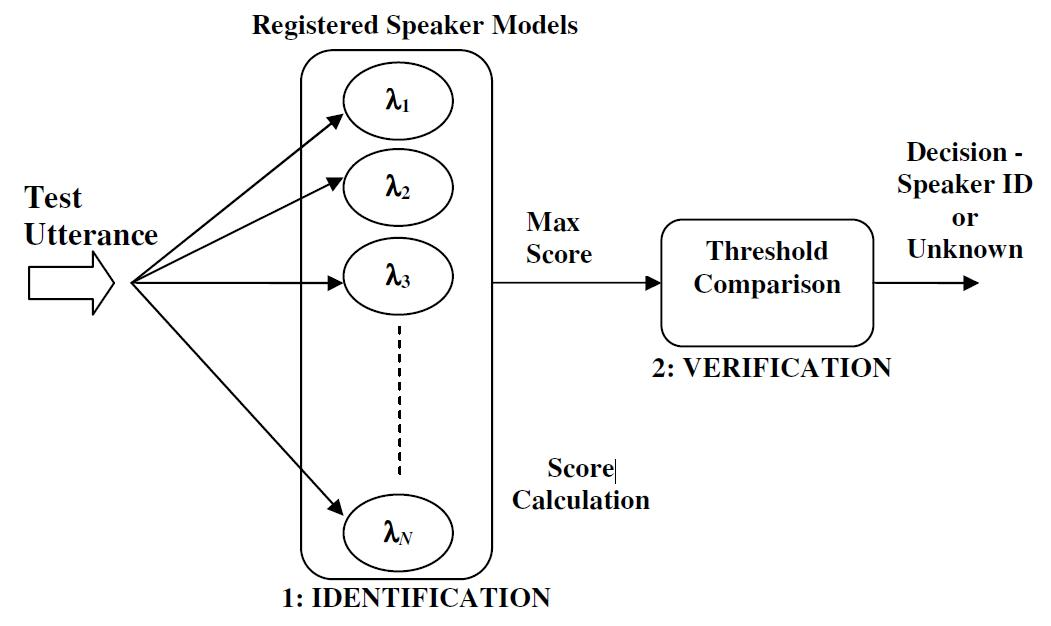
\includegraphics[scale=0.6]{image/ProcessOSIE}
	\caption{Overview of the open-set, text-independent speaker identification process}
	\label{OSIE}
\end{figure}

\begin{align}
\frac{P(\underline{b}_{test}|\lambda)}{P(\underline{b}_{test}|\lambda_{UBM})}\underset{Unknown}{\overset{Known}{\gtrless}}\gamma
\end{align}

As the Equation above, if the expected PDF from the registered model is larger than threshold ratio multiply PDF from UBM model, the speaker is one of known speakers, otherwise not. The reason why choosing UBM model for testing is that UBM model is trained from a large amount of people, so it has more universality than other registered models. Unknown speaker could have higher log-pdf in UBM model. Then we have to set up some indexes in order to evaluate the ratio test. In general, there are 3 types of error will happen in our model:

\begin{itemize}
	\item[-] a test utterance from one of registered speaker misidentified to another registered speaker, referred to Mislabelling (ML)
	\item[-] a test utterance from one of registered speaker misidentified to unknown speaker, referred to False Rejection (FR)
	\item[-] a test utterance from unknown speaker misidentified to one of registered speaker, referred to False Acceptance (FA)
\end{itemize}

So, the identification problem transfered into tradeoff problem between 3 types of error. In order to obtain the overall tradeoff performance, we set up Accumulative Error Rate (AER), it defines that

\begin{align}
AER(\varsigma)=100*\frac{ML(\varsigma)+FR(\varsigma)+FA(\varsigma)}{T}
\end{align}

where $\varsigma$ is the threshold ratio and T is the total number of test voice set. Then we applied grid-search setting up several continuous threshold ratio and calculate the Expected ML rate, FR rate, FA rate and AER respectively through cross validation.

\begin{figure}
	\centering
	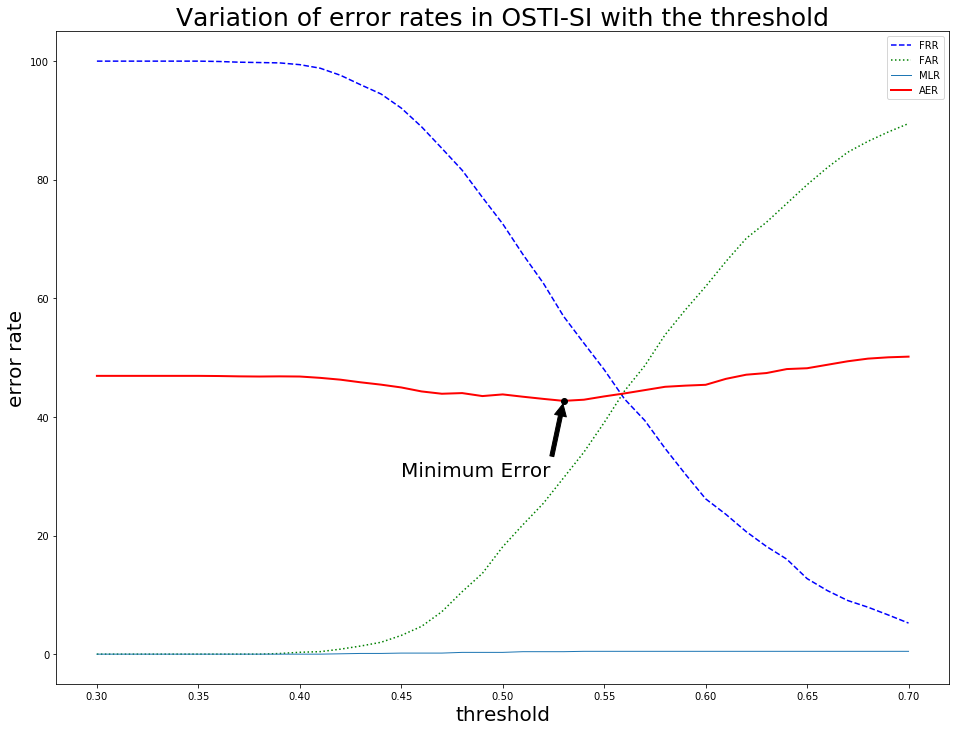
\includegraphics[scale=0.5]{image/enhancement}
	\caption{Variation of error rates in OSTI-SI with threshold}
	\label{enhancement}
\end{figure}

From the Figure.\ref{enhancement}, we got conclusion that with the threshold increasing, FA rate increases and FR rate drops. The best threshold is around 0.53 because it has minimum AER which is approximately 42\%. 

In future work , we think it is promising to replace standard UBM with UBM with score normalization or other form, setting up more benchmarks and find out the best method with lowest error rate.

\appendix
\chapter{Additionally}
You may do an appendix



% -------------------> end writing here <------------------------
% *****************************************************************
\listoffigures
\listoftables

\ifthenelse{\equal{\doclang}{german}}{
	\bibliographystyle{IEEEtran_ISSger}
}{
	\bibliographystyle{IEEEtran_ISS}
}
\bibliography{refs}

% *****************************************************************
%% Additional page with Declaration ("Eidesstattliche Erklrung");
%% completed automatically
\begin{titlepage}
      \vfill
      \LARGE \ifthenelse{\equal{\doclang}{german}}{\textbf{Erkl\"arung}}{\textbf{Declaration}}
      \vfill

      \ifthenelse{\equal{\doclang}{german}}{
         Hiermit erkl\"are ich, dass ich diese Arbeit selbstst\"andig verfasst und keine anderen als die angegebenen
         Quellen und Hilfsmittel benutzt habe.
      }
      {
         Herewith, I declare that I have developed and written the enclosed thesis entirely by myself and that I have not used sources or means except those declared.
      }

      \vspace{1cm}

      \ifthenelse{\equal{\doclang}{german}}{
         Die Arbeit wurde bisher keiner anderen Pr\"ufungsbeh\"orde vorgelegt und auch noch nicht ver\"offentlicht.
      }
      {
         This thesis has not been submitted to any other authority to achieve an academic grading and has not been published elsewhere.
      }

      \vfill

      
      Stuttgart, \signagedate
      \hfill
      \begin{tabular}{l}
          \hline
          \student
      \end{tabular}
\end{titlepage}



\end{document}
